\section{Traversing the tree}
\subsection{Concepts that come into play}
\subsubsection{`Bygg min svar'}
While traversing down our tree, we `build' our solution. But what does `building' mean?
Well, we use a \texttt{result::String()} to keep track of our progress so far. Once we hit a \texttt{:broken} branch, we add a pound (\#) to our \texttt{result}. Once we hit a \texttt{:working}, we add a period (.) to \texttt{result}.

\subsubsection{Counting broken hot springs}
How do we determine if we have the maximum number of rows in a subsection or our pattern as allowed by the clue i.e. we have matched a clue? 

Well we can use a \texttt{rows} variable to count the number of broken springs in a row. If we encounter a \texttt{:broken} spring, we increment \texttt{rows}, if we encounter a \texttt{:working} or an \texttt{:unknown} spring, then we reset \texttt{row}.
Hold that thought by the way. We will explore edge cases for this in section 3.3.

\subsubsection{Still got more clues?}
And finally, we must determine if we have `explored' all our clues. We use a \texttt{clue\_index} to determine which \texttt{clue\_element} we are currently working with.

\subsubsection{And lastly, the stack}
We also make use of a \texttt{stack}. We can implement a stack in Elixir using only four functions.

\begin{lstlisting}[language=Elixir, caption=Simple LIFO stack]
defmodule Stack do
  def push(stack, {:node, nil}) do {stack, nil} end
  def push(stack, a) do
    id = length(stack) + 1
    {[{:s_el, id, a} | stack], id}
  end
  def pop([]) do {:stack_empty, []} end
  def pop(from_stack) do
    [head | tail] = from_stack
    {head, tail}
  end
end
\end{lstlisting}

\begin{figure}
    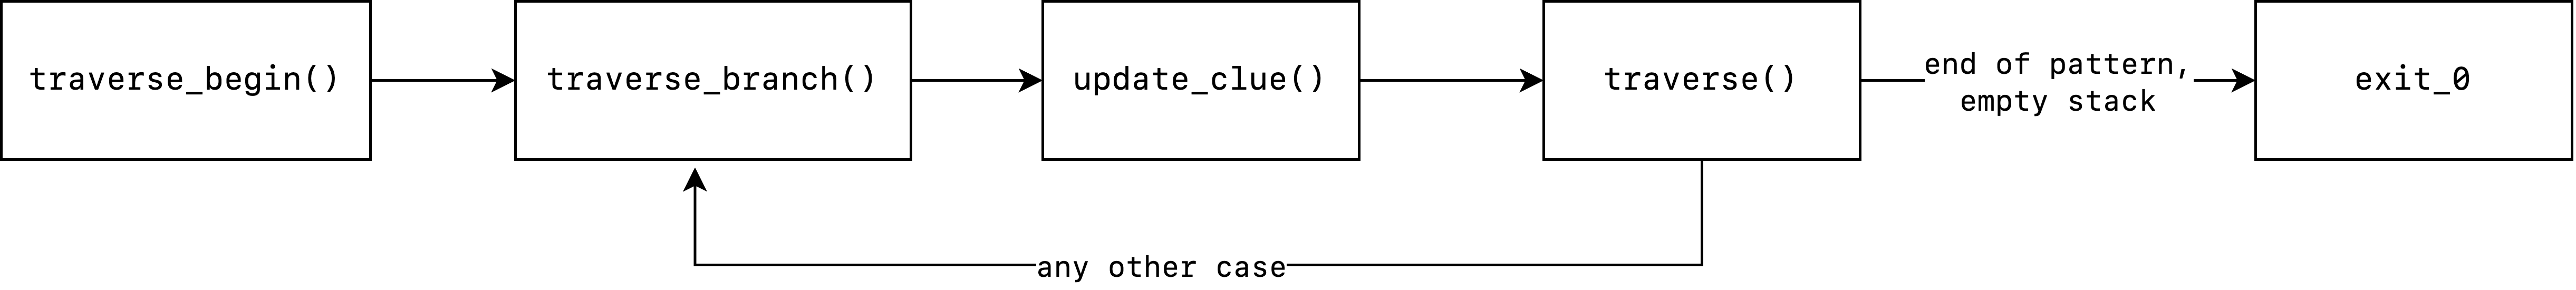
\includegraphics[width=\textwidth]{img/message_loop_h}
    \caption{Message loop}
\end{figure}

\pagebreak
\subsection{The message loop}
Recursion has been used but the recursive calls are structured in a, sort of, message loop.

\subsection{Traversing \texttt{:unknown} branch}
When encountering this branch we must (a) push our right branch into our stack (we can ignore if our right branch is a \texttt{nil} as our stack already handles it for us)
and (b) traverse down the left stack. We do not increment our \texttt{rows}, we do not update our \texttt{clue\_index}.

\begin{lstlisting}[language=Elixir, caption=Example of how a branch is traversed]
def traverse_branch({:n, :un, left, {:n, nil}}, {:d, clue, c_in, rw, res}, stack) do
    traverse(left, {:d, clue, c_in, 0, res <> "."}, Stack.push(stack, {:st_el, {:n, :b, {:n, nil}, {:n, nil}}, rw, res}))
  end
\end{lstlisting}

\subsubsection{Edge cases}
What happens when \texttt{rows == clue\_element}? Well, that means a right branch (a broken branch) at this stage would result in an erroneous solution. We must, therefore, force-traverse the left branch.

\begin{lstlisting}[language=Elixir, caption=Edge case ignoring the right branch]
def traverse_branch({:n, :u, l, _}, {clue, ci, true}, {_, _}, {rw_pat, res, _}, stack) do
  update_clue(l, {clue, ci, true}, {0, false}, working_res(rw_pat, res), stack)
end
\end{lstlisting}

\subsection{Traversing a \texttt{:broken} and \texttt{:working} branch}
Pretty straightforward. Hit a \texttt{:working}? Go left. Hit a \texttt{:broken}? Go right.

\subsubsection{Edge cases}
No edge cases. These functions behave nicely and are well-trained.

% Let's say our \texttt{rows == clue\_element}. Well, we have reached the maximum number of rows that we can afford to have. This is a dud end so we must discard and restart from our stack.

% Our second edge cases is when we have already `explored all our clues'. \textbf{Note}: we can check this by simply doing \texttt{length(clue) == clue\_index}. This also means a dud end and we must restart from the stack.

\subsection{The deal with the clues}
All of our \texttt{traverse\_branch()} methods call the \texttt{update\_clue()} method. Update clues essentially checks if the \texttt{rows} equals the maximum number allowed. But not without it's edge cases it doesn't.

\subsubsection{Rows allowed met but left node is \texttt{nil}}
We are expected to take a left branch when our \texttt{rows} reaches maximum allowed. But what happens if our left node is \texttt{nil}. Well, this means we have reached a dud end and we must restart traversing from our stack.

\begin{lstlisting}[language=Elixir, caption={\texttt{update\_clue() when left node is \texttt{nil}, maximum rows have been reached}}]
def update_clue({:n, _, {:n, nil}, _}, {clue, clue_index, _}, {_, true}, {rw_pat, res, _}, stack) do
    traverse({:n, nil}, increment(clue, clue_index), {0, false}, {rw_pat, res, true}, stack)
end
\end{lstlisting}


\subsubsection{Forcing a left traversal}
When we have reached the maximum number of rows (and our left branch is not \texttt{nil}), we must force traversal down the left node. We simply ignore that the right branch exists, no adding to any stack.

\begin{lstlisting}[language=Elixir, caption={\texttt{update\_clue()} Forced left-branch traversal}]
def update_clue({:n, :u, l, _}, {clue, clue_index, _}, {_, true}, {rw_pat, res, _}, stack) do
    traverse_branch(l, increment(clue, clue_index), {0, false}, working_result(rw_pat, res), stack)
end
\end{lstlisting}

\subsection{The \texttt{traverse} method}
The role of the \texttt{traverse} method is to determine if our program should continue execution or exit out of recursion. 

If we have reached the end of our pattern (meaning the length of our \newline \texttt{raw\_pattern} equal \texttt{result}) and our stack is also empty, well then we've had a good run but it's time for exit code 0.

If we have reached the end of our pattern (meaning the length of our \newline \texttt{raw\_pattern} equal \texttt{result}) and our stack still has elements in it, we go check them out! We have a stack traversal. We can also take this opportunity to see if the result we have in hand is a valid or a failed result (we can make this check by seeing if our clues have been fully explored and our \texttt{clue\_index} == length of our clues list.)

In any other case, things will be normal and we can continue our recursive excursion by calling \texttt{traverse\_branch()}.